% PREAMBLE
\documentclass{article}
\usepackage{amsmath}
\usepackage{indentfirst}
\usepackage{graphicx}
\usepackage{hyperref}
\usepackage{caption}
\usepackage{subcaption}

\hypersetup{
  colorlinks   = true,    % Colours links instead of ugly boxes
  urlcolor     = blue,    % Colour for external hyperlinks
  linkcolor    = blue,    % Colour of internal links
  citecolor    = red      % Colour of citations
}
\title{Beerxels \\
	\large A Personal Project Report}
\author{Jonas Stolle}
\date{\today}
% DOCUMENT
\begin{document}

\begin{titlepage}
\maketitle
\centering
	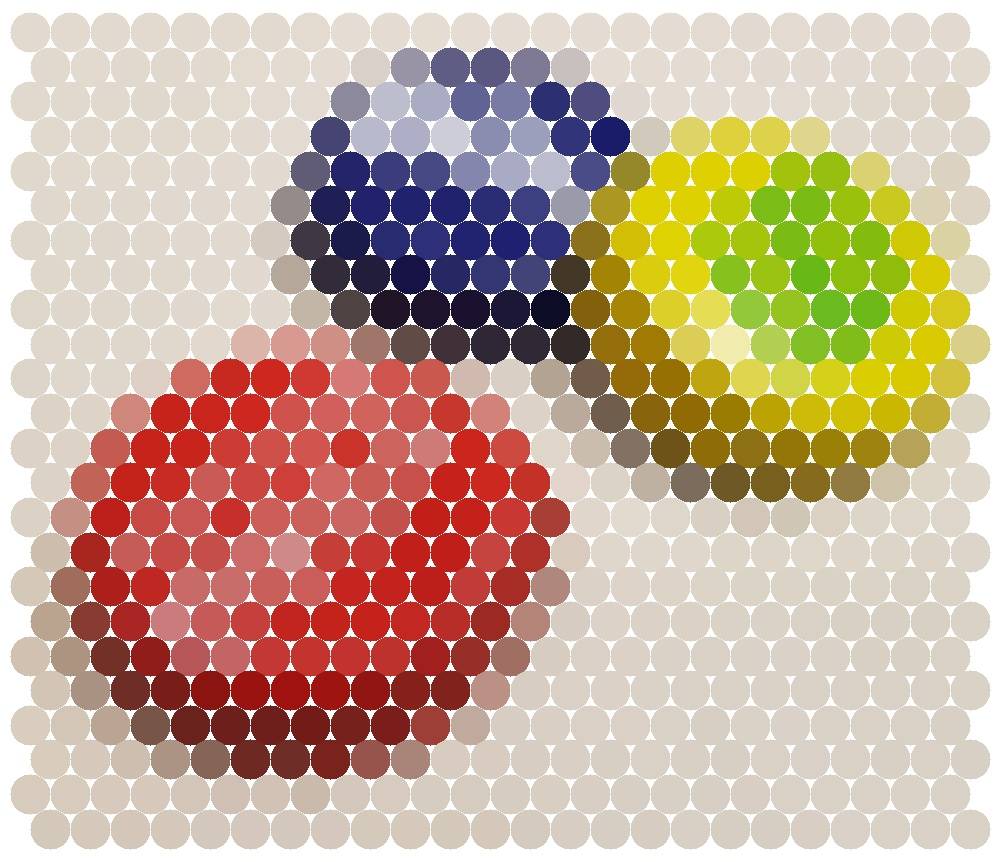
\includegraphics[width=0.8\linewidth]{caps_pics-circles.jpg}
\end{titlepage}

\section{Abstract}
This report describes the process of creating pixel art using a set of collected bottle caps. The bottle caps are captured digitally, cut out with the help of the Circle Hough Transform and an averaged color is extracted. A given reference image is tiled for the bottle caps to fit and colors are extracted yet again. Optimal pairings between the two sets are computed using the Hungarian Algorithm, with which the correct bottle cap placements are found. Finally, the physical piece is assembled by attaching the bottle caps to a metal sheet using small magnets. 

\section{Introduction}

Over the past years a rather large collection of unique bottle caps was collected which invited for a creative application. 
The idea of creating pixel art arose, i.e. the tiling of an image with caps such that in each position the color of the cap best matches the color of the underlying part of the image. This results in a downsampled but recognizable version of the reference image. Finding the correct cap placements may be attempted by hand, but the approach of choice is to find a solution via computational means.
\section{Methods}
This section details the process of going from a set of bottle caps to the finished piece.
\subsection{Data Acquisition}
For a start, the bottlecaps and the reference image need to be available in digital form. While the latter is assumed to be given as such, the bottle caps are each captured using a digital camera in consistent lighting conditions. To aid with preprocessing, the background is chosen to be a white sheet of paper on which the bottle caps are placed within a circular black area just slightly larger than the caps themselves.  
\begin{figure}[h]
	\begin{center}
	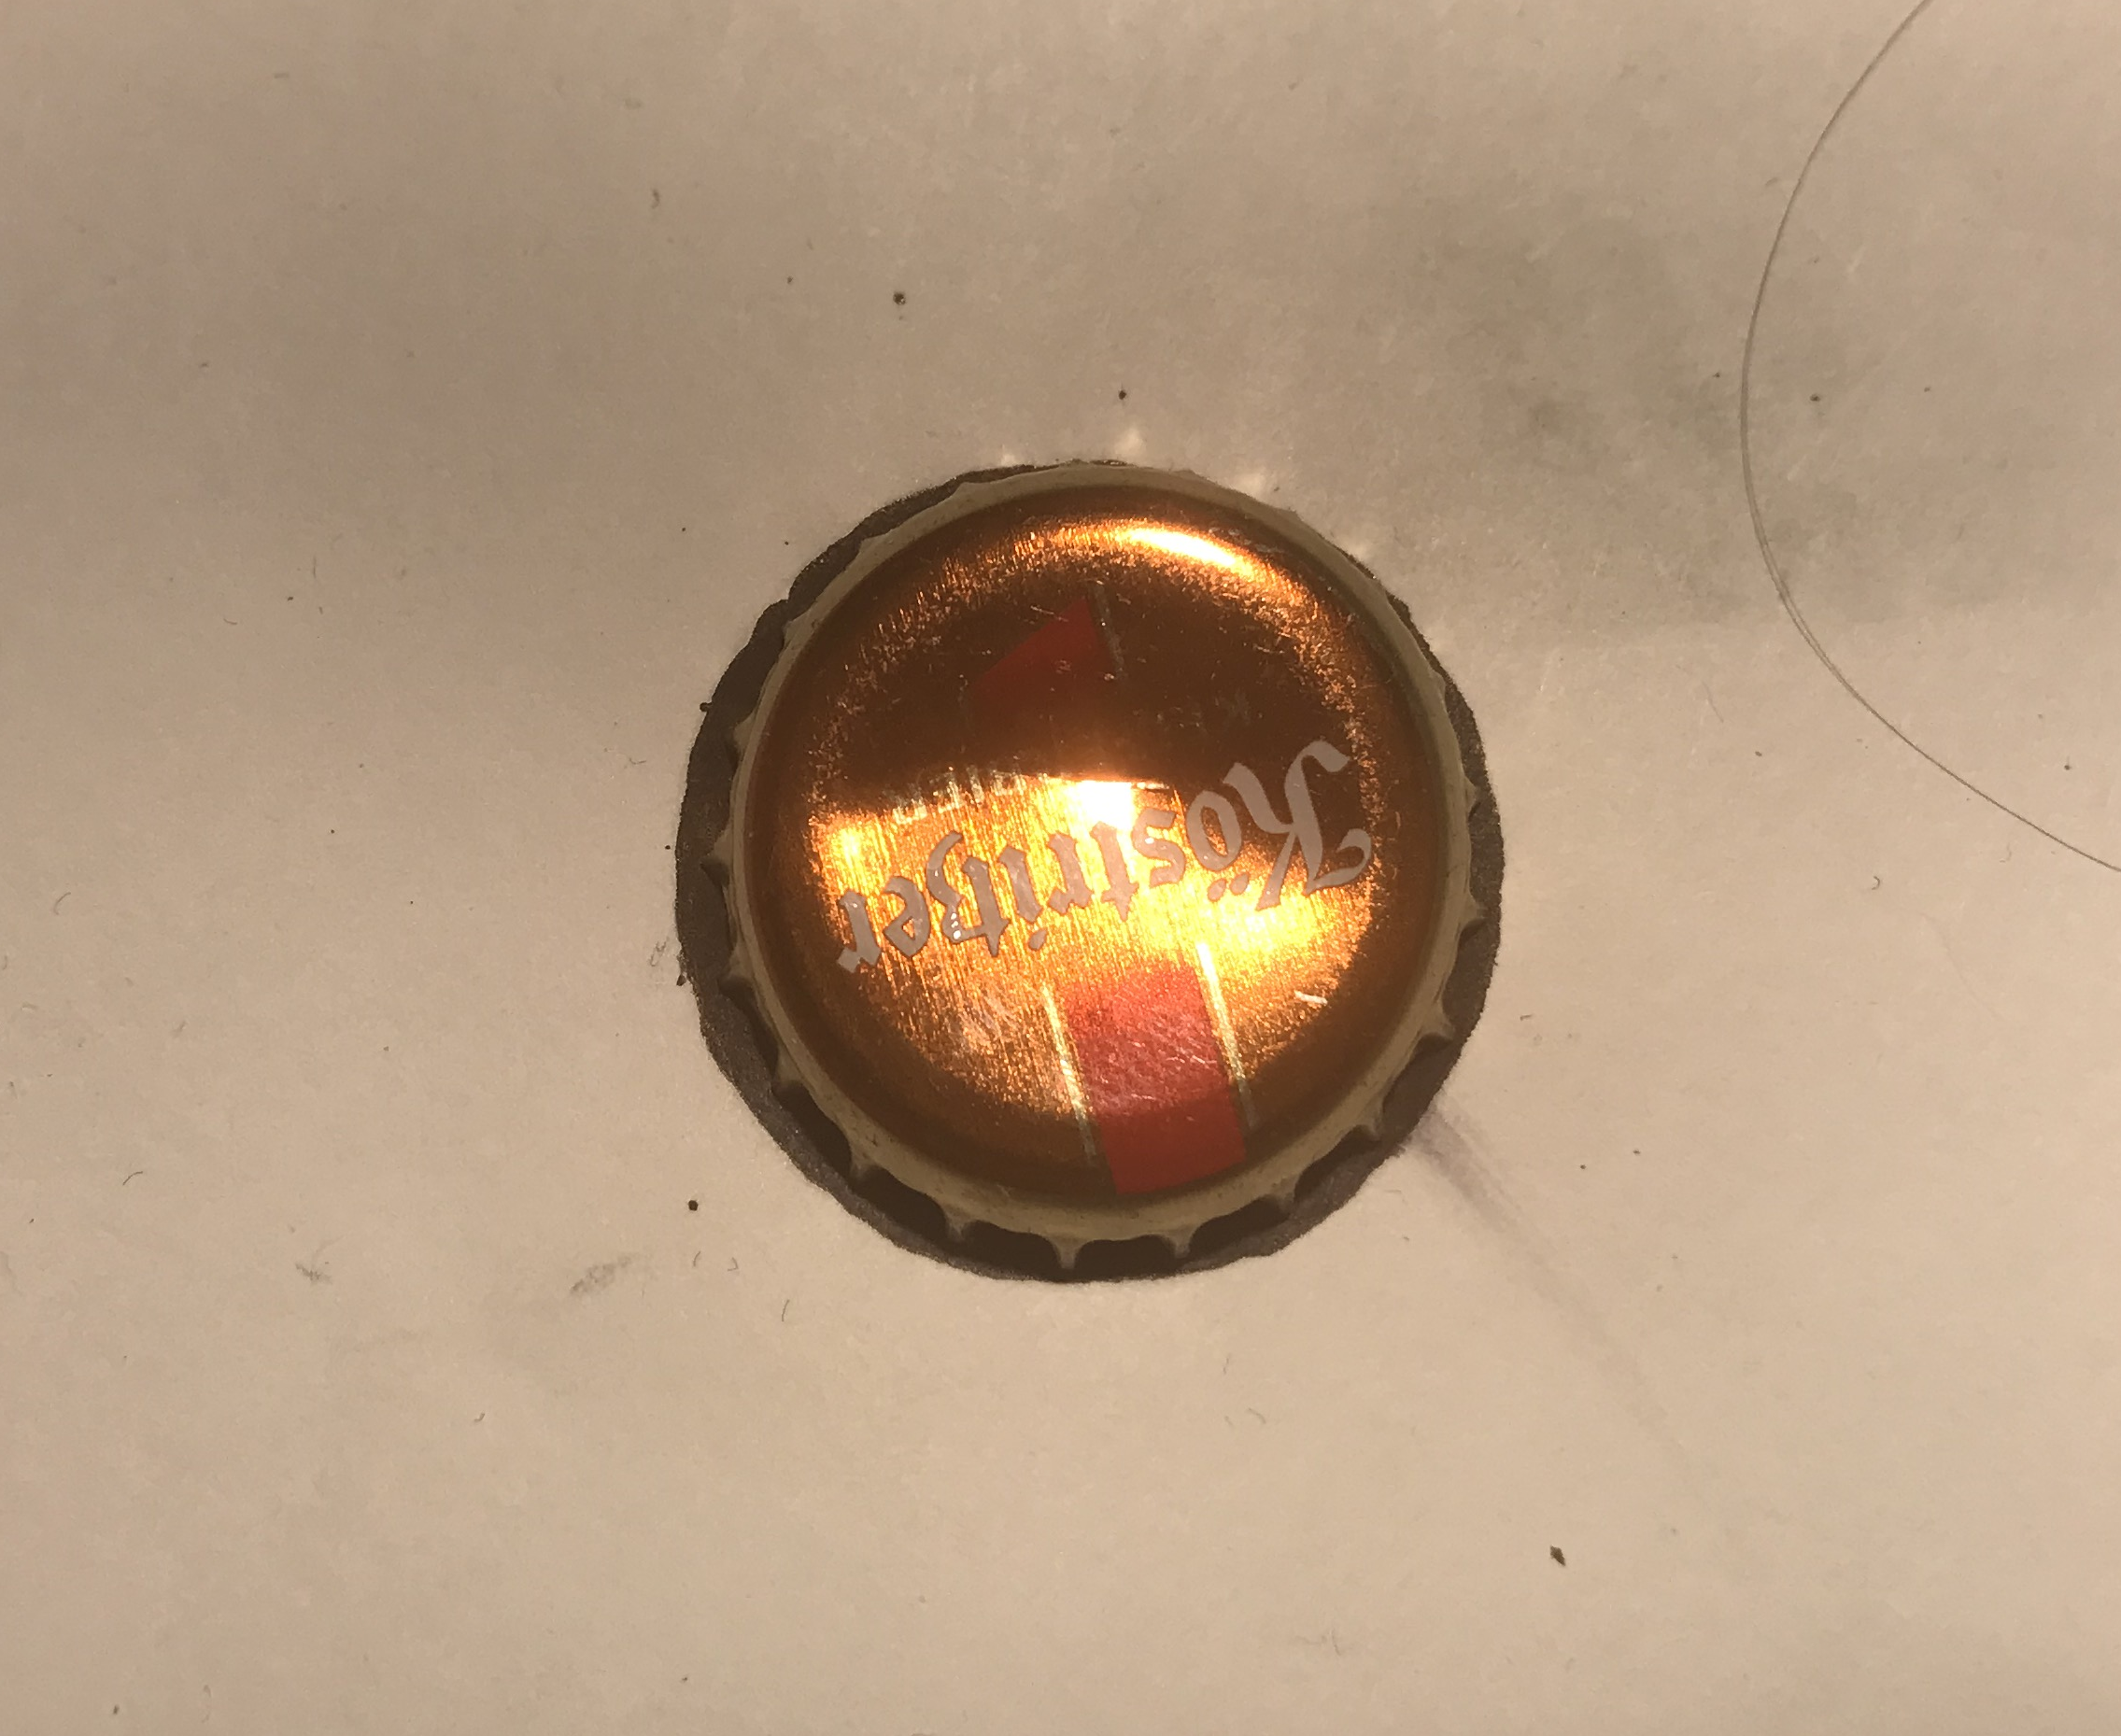
\includegraphics[width=0.5\linewidth]{cap_raw.png}
	\caption{Raw captured image of bottle cap on a whit sheet of paper. Notice the black area within which the cap is positioned.}
	\label{cap:raw}
\end{center}
\end{figure}
\subsection{Preprocessing}
To set up the problem, the colors to eventually be matched need to be extracted from both the bottle caps and the reference image. The process of computing the colors is identical for both cases, but the method of finding the appropriate locations to do so differs.
\subsubsection{Bottle Caps} \label{caps}
Here it is assumed that every image contains only a single bottle cap, which must first be located precisely. 
This can be achieved using an implementation of the Circle Hough Transform \cite{DAVIES198837}, which returns a list of circles, parametrized by their center point positions and radii, which are sorted by the confidence of the algorithm. 
The goal is to detect the outline of the black area, which  will most likely have the highest confidence, as the high contrast between the black and white parts is favorable for the detection algorithm. Thus the first entry in the list is chosen as a close approximation to the outline of the bottle cap.
\begin{figure}[h]
        \begin{center}
        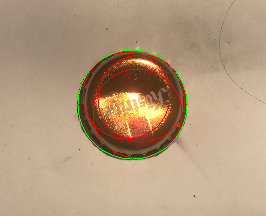
\includegraphics[width=0.5\linewidth]{cap_hough.png}
	\caption{The same bottle cap image as in \ref{cap:raw}, with the circles returned from the Circle Hough Transform as an overlay. The green circle has the highest algorithmic score and does match the outline of the bottle cap very closely.}
        \label{cap:hough}
\end{center}
\end{figure}
  
Also note that the algorithmic parameters need to be tuned for good results. 
Given the correct circle parameters, the bottle cap is then cut out and its averaged color is computed. 
\begin{figure}[h]
        \begin{center}
        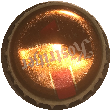
\includegraphics[width=0.3\linewidth]{cap_cutout_white_2.png}
	\caption{Cutout of the bottle cap presented in \ref{cap:raw} and \ref{cap:hough}.}
        \label{cap:cut}
\end{center}
\end{figure}

As colors on computers are generally represented in terms of their red, green and blue components (RGB), the average of each component needs to be computed for the final averaged color of the bottle cap.
The reasoning for the average as a metric are its ease of implementation and its rotational symmetry, which allows the caps in the physical piece to be placed in any orientation desired. 
The set of all extracted colors is then stored in a vector $\boldsymbol{v}_{caps}$, with each element containing the red, green and blue components.

\subsubsection{Reference Image}
Before any colors can be extracted from the reference image, an appropriate tiling needs to be computed on it, as it determines the positions of the bottle caps in the final piece. In this project the tiling is understood as a repeating pattern of non-overlapping circles covering the reference image. 
An important constraint here is the number of available bottlecaps $n_{caps,max}$, which limits the number of circles $n_{caps,piece}$ the tiling may use to cover the image.  
\begin{equation}
\label{eqn:max}
n_{caps,piece} \leq n_{caps,max} 
\end{equation}
While a quadratic (grid like) tiling would be the easiest to compute, a hexagonal pattern is chosen because of its dense packing and the authors aesthetic preference. Given the centerpoint $(x_c,y_c)$ of a circle and its radius $r$, the rule for finding adjacent circles in the tiling is as follows:
\begin{equation}
\label{eqn:adj}
(x,y)_{adj} = 
	\begin{cases}
		\{(x_c \pm 2r,y_c)\} \text{ for horizontal neighbors,} \\
		\{(x_c \pm r, y_c \pm \sqrt{3}r)\} \text{ for vertical neighbors.} \\
	\end{cases}
\end{equation}
Notice that \ref{eqn:adj} depends only on the $r$ chosen. 
Let $tile(r):\ r\ \rightarrow \{(x,y)\}$ be a function that covers the plane following \ref{eqn:adj}.
Assuming the reference image lies within a rectangular set of points 
\begin{equation}
	D = \{(x,y)\ \vert\ x \in [0,x_{bound}], y \in [0,y_{bound}]\},
\end{equation}
the following optimization problem can be formulated:
\begin{equation}
\label{eqn:tile}
\begin{aligned}
& \ \boldsymbol{\max_{r}}\ \ \ \vert tile(r) \vert \\
& \ \ \textbf{s.t.}\ \ \  \{(x,y)\}\ \ \subseteq\ D  \\
& \ \ \ \ \ \ \ \ \ \vert \{(x,y)\} \vert\ \leq\ n_{caps,max}, \\
\end{aligned}
\end{equation}
where $\vert(\cdot)\vert$ is read as the number of elements in $(\cdot)$.


In practice this is solved by iterating the radius from a starting size of 3 pixels, covering the reference image each time and checking whether for the total number of circles required \ref{eqn:max} holds. The first radius to not violate this constraint is then the optimal solution to \ref{eqn:adj}.
\begin{figure}[h]
        \begin{center}
        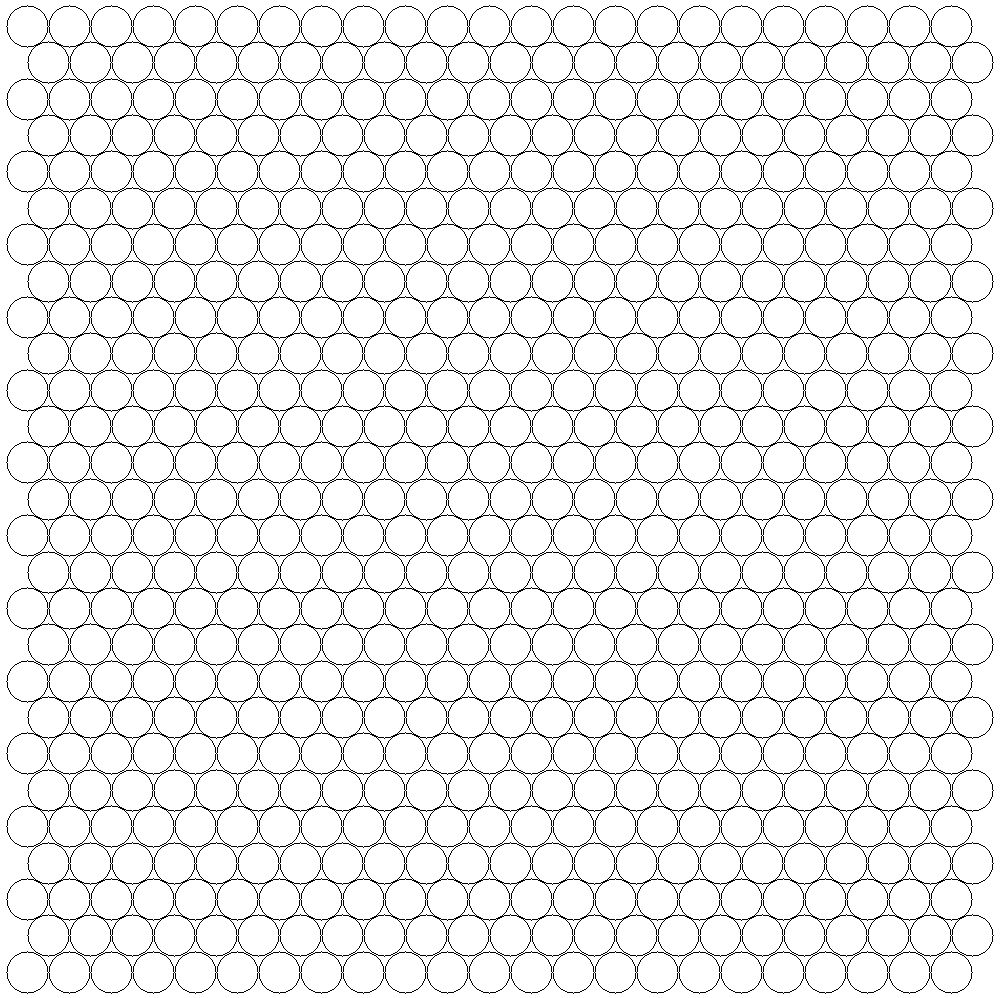
\includegraphics[width=0.4\linewidth]{optimal_tiling.png}
        \label{opttile}
	\caption{Visualization of an optimal tiling solution to problem \ref{eqn:tile}, with a $n_{caps,max} = 628$ and $n_{caps,piece} = 621$.}
\end{center}
\end{figure}
Note that in the general case not all bottle caps will be used, but that number will always remain relatively small compared to the size of the entire set of caps.
With the positions of the bottle caps in the refernce image being known, for every circle the averaged color is computed analogously to \ref{caps} and stored in a vector $\boldsymbol{v}_{ref}$. 
 
\subsection{Matching}
Given the averaged colors of all the bottlecaps, the matching process can begin. Concretely pairings need to be found between all elements $v_{caps}$ and $v_{ref}$ of $\boldsymbol{v}_{caps}$ and $\boldsymbol{v}_{ref}$ respectively, such that in each pair the colors are as "similar" as possible. This similarity is computed via the
\begin{equation}
\label{eqn:ssd}
	\text{Sum of Squared Deviations} = \sum_{i = 1}^{3} (v_{caps,i}-v_{ref,i})^2 ,
\end{equation}
where $i = \{1,2,3\}$ corresponds to the RGB components of each color.
This is a Balanced Assignment Problem and can be solved using the Hungarian Algorithm \cite{https://doi.org/10.1002/nav.3800020109}, of which numerous implementations are readily available. 
The algorithm returns the optimal pairings w.r.t. \ref{eqn:ssd}, with which the bottle caps can be placed in their corresponding positions.
\subsection{Physical Implementation}
Using the digital version of the piece as a template, the reference image is recreated in a jigsaw like fashion using the bottle caps in the real world. The canvas is chosen to be a magnetic sheet of metal, to which every bottlecap is fixed using small neodymium magnets. This makes the bottle caps removable and leaves the possibility open to change the design in the future.
\section{Results} \label{results}
This section presents the finished piece in both its digital and physical form.

\begin{figure}[h]
	\centering
	\begin{subfigure}[t]{0.3\linewidth}
		\centering
	        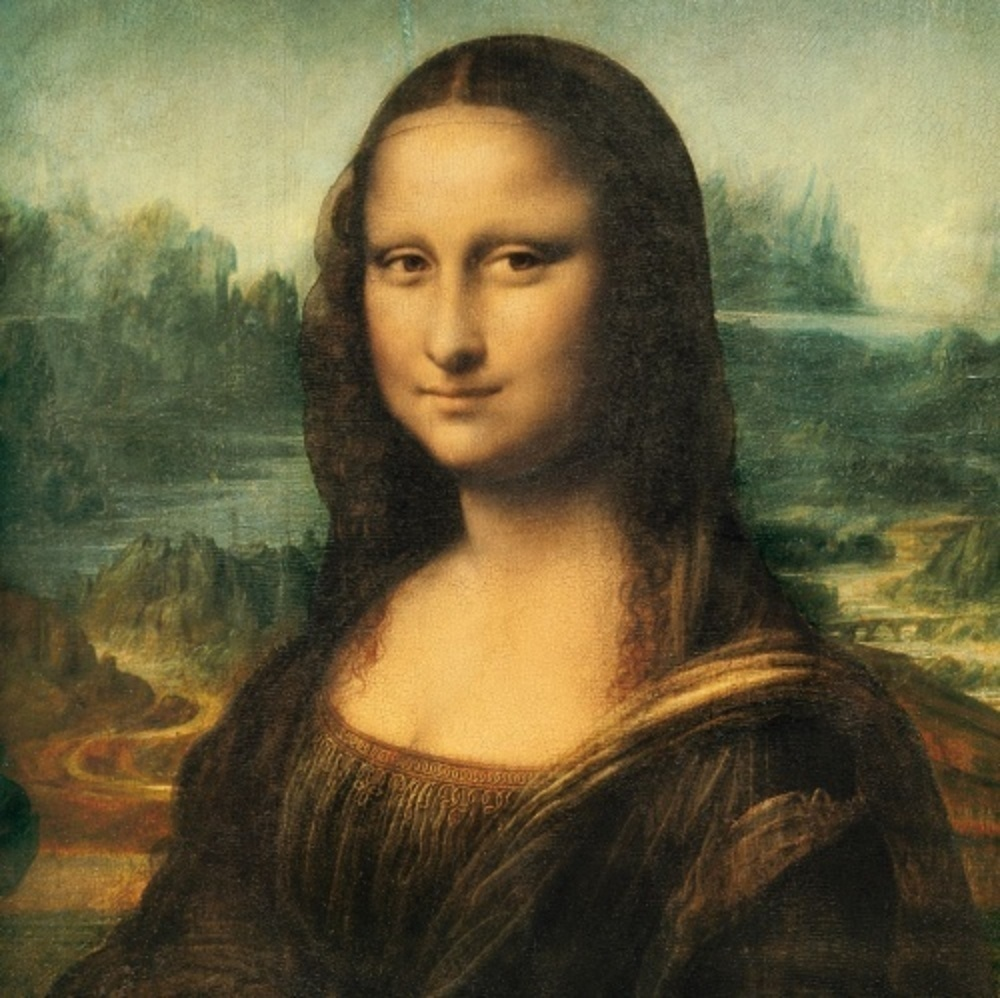
\includegraphics[width=\linewidth]{mona-lisa.jpg}
		\caption{A moderately well known painting which is used as the reference image.}
		\label{fig:mona1}
	\end{subfigure}
	\hfill
	\begin{subfigure}[t]{0.3\linewidth}
		\centering
		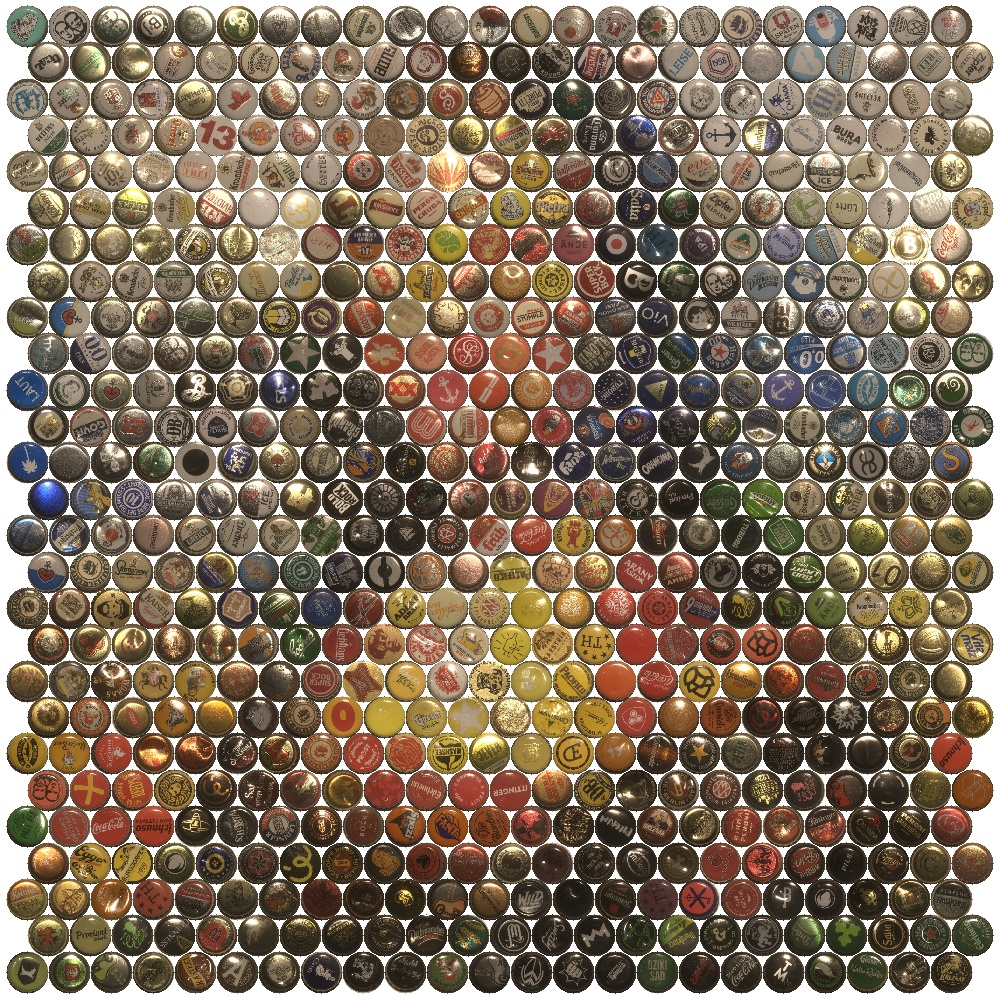
\includegraphics[width=\linewidth]{mona-lisa-caps-white.jpg}
		\caption{Digital version of the finished piece.}
		\label{fig:mona2}
        \end{subfigure}
	\hfill
        \begin{subfigure}[t]{0.3\linewidth}
		\centering
		\includegraphics[width=\linewidth]{mona-lisa-caps-real.jpg}
		\caption{Physical version of the finished piece.}
		\label{fig:mona3}
        \end{subfigure}
\end{figure}
For increased visual enjoyment, it is advised to view this document from further away or to squint ones eyes slightly. 

\section{Discussion} \label{discussion}
Clearly, the quality of the image does detiriorate with every processing step, however the impression of the reference image persists throughout to the final piece. 
The bright region at the top left of \ref{fig:mona2} is predominantly made up of caps with strong reflections, which does not translate well to the physical piece \ref{fig:mona3} as they appear noticably dimmer without the reflections present.
Better results will likely be achieved with more accurate capturing of the bottle caps. Possible approaches here could be more diffuse lighting conditions, which would reduce problematic reflections, or the use of a polarized filter, with similar effect.
Another issue encountered were inaccuracies with the circle detection as it did not always work perfectly, especially when the design of the bottle caps featured high contrast circles. In most cases however, the averaged color of a section is still close to that of the full bottle cap, or at least the error is small enough to not be noticable in the result. 
Still, a remedy for this would be to manually verify and potentially tune the detected circles manually at the preprocessing stage. 
Also note that the set of bottle caps fundamentally dictates the color accuracy of the piece. For \ref{results}, a non-negligible set of red bottle caps was available and most of them were used for the final piece. As a consequence, the color spectrum with respect to the reference, which has almost no red hues, is distorted. Choosing a fitting reference image with a color distribution similar to that of the bottle caps will help with this issue. 

Despite its shortcomings, this project is ultimately artistic in nature and the quality of the results lies in the eye of the beholder.
\bibliographystyle{abbrv}
\bibliography{refs}
\end{document}
